%!TEX root = ../dokumentation.tex

\chapter{Implementierung der Knoten}

\section{Knoten-Arten}
Der Kern der Applikation bilden die verschiedenen Knoten: Mit ihnen kann das Modell aufgebaut werden. Dabei ist es wichtig, dass die Knoten die verschiedenen Anwendungsfälle abdecken.

Um herauszufinden, welche Knoten-Arten benötigt werden, wurden mehrere Beispiel-Modelle durchgespielt und evaluiert, mit welchen Knoten diese sich am besten umsetzen lassen.

Wohnungsbeispiel:
\begin{algorithm}[H]
    \caption{Beispielmodell Wohnungspreise}
    \begin{algorithmic}[1]
        \State Fläche = ZufallGauss($\mu = 80$, $\sigma = 20$)
        \State a = Mathematik(Division, $\textrm{Fläche}$, $40$)
        \State b = ZufallDiskret($-1: 10\%, 0: 80\%, 1: 10\%$)
        \State c = Mathematik(Addition, $a$, $b$)
        \State Räume = Mathematik(Maximum, $c$, $1$)
        \State d = $\textrm{Fläche} \cdot 2500 + 250 \cdot \textrm{Räume}$
        \State Preis = ZufallProzentual($d$, $5\%$)
    \end{algorithmic}
\end{algorithm}

Die Knoten lassen sich in folgende Kategorien unterteilen:
\begin{itemize}
    \item \textbf{Werteknoten} können benutzt werden, um den gleichen Wert an verschiedene andere Knoten weiterzugeben. Es gibt sie für die Datentypen \textit{Boolean}, \textit{Number} und \textit{String}. Zusätzlich gibt es den Index-Knoten. Dieser gibt den aktuellen Index innerhalb des Berechnungsprozesses aus. Wird ein Wert nur für einen Knoten verwendet, kann dieser in der Regel direkt an der Eingangsschnittstelle des entsprechenden Knotens eingestellt werden; ein Werteknoten muss dafür nicht verwendet werden.
    \item \textbf{Zufallsknoten}
    \begin{itemize}
        \item \textbf{Gleichverteilung} mit einstellbarem Minimum und Maximum
        \item \textbf{Normalverteilung} mit einstellbarem Mittelwert $\mu$ und Standardabweichung\nobreakspace $\sigma$
        \item \textbf{Exponentialverteilung} mit einstellbarem $\lambda$
        \item \textbf{Anpassbare Verteilung}: Bei diesem Knoten kann die Wahrscheinlichkeitsdichtefunktion über einen grafischen Editor eingestellt werden. Die Wahrscheinlichkeitsdichtefunktion kann sowohl diskret als auch stetig sein.
        \item \textbf{Prozentuale Abweichung}: Dieser Knoten nimmt einen Wert und addiert einen zufälligen Wert zwischen $\pm \, \, inputValue \cdot \frac{percentage}{100}$
    \end{itemize}
    \item \textbf{Berechnungsknoten}
    \begin{itemize}
        \item \textbf{Mathematik}: Der Mathematikknoten wendet eine einstellbare mathematische Funktion, wie zum Beispiel Addition, Division oder trigonometrische Funktionen auf ein oder zwei Eingabedaten an
        \item \textbf{Funktion}: Der Funktionsknoten kann benutzt werden, um eine beliebige Funktion in JavaScript zu implementieren. Alle Eingangswerte werden im \texttt{this} Objekt zur Verfügung gestellt. Der Code muss ein Objekt zurückgeben, welches die Namen der Ausgangsschnittstellen als Keys und die dazugehörigen Werte enthält.
        \item \textbf{Boolean}: Dieser Knoten vergleicht zwei numerische Werte und gibt das Resultat des Vergleichs aus.
        \item \textbf{Stringlist}: Der Stringlist-Knoten erlaubt es, einen String aus einer vorgegebenen Liste von Strings auszuwählen. Welcher String ausgegeben wird, kann über die Index-Eingangsschnittstelle gesteuert werden (die Indizes beginnen bei 0)
    \end{itemize}
    \item \textbf{Bedingungsknoten}: Bedingungsknoten können genutzt werden, um sicherzustellen, dass Ausgabedaten bestimmte Bedingungen erfüllen. Wenn an der Eingangsschnittstelle der Wert \texttt{false} anliegt, wird der aktuelle Datenpunkt neu berechnet.
    \item \textbf{Ausgabeknoten}: Jeder Ausgabeknoten repräsentiert eine Spalte in den generierten Ausgabedaten. Der Name der Spalte kann im Textfeld des Ausgabeknotens gesetzt werden.
\end{itemize}

\section{Anpassbare Verteilung}
\label{sec:anpassbareverteilung}

Steht man vor der Aufgabe Daten zu generieren, die von Zufallswerten einer komplexen Wahrscheinlichkeitsverteilung abhängen, besteht das Problem, dass mit den standardmäßigen Verteilungen oft keine passende Wahrscheinlichkeitsverteilung gefunden werden kann. 

In dem Fall soll der Benutzer in der Lage sein, schnell und einfach mit einer grafischen Oberfläche eine gewünschte Wahrscheinlichkeitsverteilung zu modellieren. Dadurch wird zum einen eine konzeptuelle Umgebung geschaffen, als auch der Aufwand erspart eine exakte Dichtefunktion der Wahrscheinlichkeitsverteilung zu entwerfen. Selbst wenn es keine exakte Dichtefunktion für die Wahrscheinlichkeitsverteilung gibt, könnte sie mit diesem Node näherungsweise modelliert werden.

Da dieser Knoten deutlich größeren Implementierugnsaufwand im Vergleich zu den anderen Knoten benötigt, soll in diesem Kapitel näher auf dessen Umsetzung eingegangen werden. Die anpassbaren Zufallsknoten bestehen aus den zwei Komponenten: 
\begin{enumerate}
    \item Grafische Modellierung der Wahrscheinlichkeitsverteilung
    \item Erzeugung der Zufallszahl
\end{enumerate}

In diesem Kapitel soll auf die grafische Modellierung einer Wahrscheinlichkeitsverteilung eingegangen werden. Wie aus der modellierten Wahrscheinlichkeitsfunktion eine Zufallszahl generiert werden kann, wird in der Theorie im Kapitel \ref{sec:anpassbareverteilungberechnung} (S. \pageref{sec:anpassbareverteilungberechnung}) behandelt.

\subsection{Grafische Modellierung einer Wahrscheinlichkeitsverteilung}

\todo{Bilder wies tatsächlich aussieht?}
Für die grafische Oberfäche der beiden Nodes wird ein freier Zeichenraum benötigt, auf dem das Linien- und Säulendiagramm gezeichnet werden kann. Zudem soll die Oberfläche Interaktionsmöglichkeiten zur Gestaltung der Verteilung geben. Da es bereits einige Implementierungen von Visualisierungsmöglichkeiten in JavaScript gibt, wird auch an dieser Stelle an eine bereits existierende Lösung zurückgegriffen. Hierfür wird das JavaScript Framework Chart.js verwendet aus den folgenden Gründen \cite{chartjs}:
\begin{itemize}
    \item Open-Source + MIT License: Freie Nutzung ohne anfallende Kosten
    \item Unterstützung von 8 Chart-Typen: Inklusive Linien- und Säulendiagramm
    \item HTML5 Canvas: Gute Rendering Performanz
    \item Responsive: Diagramme werden in einer skalierbaren Sidebar verwendet
\end{itemize}

Für die stetige Wahrscheinlichkeitsverteilung müssen in dem Liniendiagramm Interaktionsmöglichkeiten zum Hinzufügen (Doppelklick), Löschen (Rechtsklick) und Verschieben (Linkslick) von Punkten implementiert werden. Die Punkte sind durch eine Linie miteinander verbunden. Im linearen Modus werden zwei aufeinanderfolgende Punkte mit einer Geraden verbunden.

Das Säulendiagramm für die diskrete Wahrscheinlichkeitsverteilung soll dem Nutzer die Möglichkeit geben die einzelnen Säulenhöhen zu setzen (Linksklick). Ein wichtiges Detail ist bei dem Setzen der Säulenhöhen, dass dies auch funktionieren soll, wenn der Zeiger sich bei gehaltener Taste über mehrere Säulen bewegt, weil die Gestaltung des Verteilungsdiagramms sonst bei einem großen Wertebereich sehr aufwändig wird. 

\begin{figure}[H]
    \center
    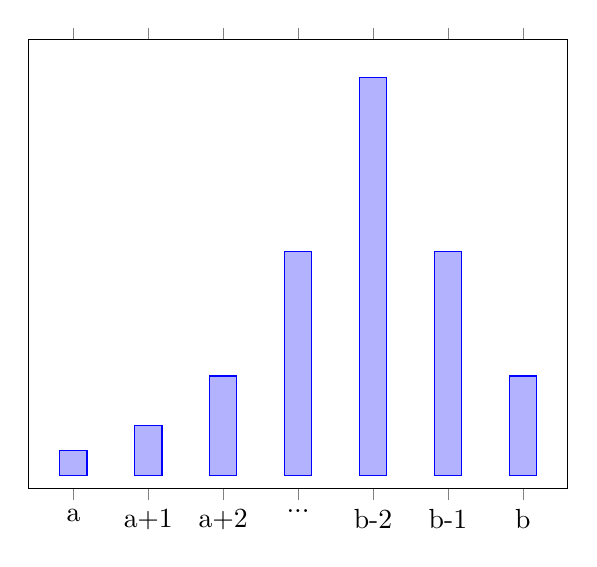
\begin{tikzpicture}
        \begin{axis}[
                ybar, 
                ytick=\empty,
                symbolic x coords={a,a+1,a+2,...,b-2,b-1,b},
            ]
            \addplot plot coordinates
                {(a,1) (a+1,2) (a+2,4) (...,9) (b-2,16) (b-1,9) (b,4)};
        \end{axis}
    \end{tikzpicture}
    \caption{Darstellung einer diskreten Verteilung}
\end{figure}

Sei der Wertebereich definiert durch die Werte $a,a+1,a+2,\dots,b-2,b-1,b$ im Intervall $[a,b]$, wobei $a,b \in\mathbb{N}_0$, $x_0 \le x_n$, dann werden genau $b-a+1$ Klicks benötigt, wenn alle Säulen gesetzt werden sollen. Der Aufwand könnte erheblich reduziert werden, indem im Optimalfall mit einem einzigen haltenden Klick und einer Bewegung des Zeigers alle Säulen gesetzt werden können.

Ein Problem bei dieser Funktion ist, dass oft nicht alle Säulen auf die Zeigerposition gesetzt werden, weil das mouseover-Event nicht oft genug auslöst. Dies wird durch mehrere Faktoren negativ beeinflusst:
\begin{itemize}
    \item Niedrige Skalierung des Diagramms
    \item Hohe Zeigergeschwindgkeit in horizontaler Richtung
    \item Großes Intervall $[a,b]$
 \end{itemize}

Um diesem Effekt entgegenzuwirken, kann eine Schätzung der Mausbewegung mithilfe einer linearen Interpolation vorgenommen werden. Dazu muss bei jedem Handleraufruf für das mouseDown-Event die aktuelle Position des Zeigers gespeichert werden. Der Handler für das mouseMove-Event hat dann immer die Koordinaten für die letzte und aktuelle Position des Zeigers. Seien die beiden Punkte $A(a_x|a_y), B(b_x|b_y)$ gegeben, dann ist die lineare Interpolationsfunktion für alle diskreten Werte im Intervall $[a_x,b_x]$ definiert als $f(x)=mx+a_y-m*a_x$ mit $m=\frac{b_y-a_y}{b_x-a_x}$. Alle Säulen zwischen der letzten bekannten und der aktuellen Zeigerposition können nun gesetzt werden, sodass keine Lücken mehr beim Bearbeiten der diskreten Wahrscheinlichkeitsverteilung auftreten.